\documentclass[11pt,a4paper]{report}
\usepackage[textwidth=37em,vmargin=30mm]{geometry}
\usepackage{calc,xunicode,amsmath,amssymb,paralist,enumitem,tabu,booktabs,datetime2,xeCJK,xeCJKfntef,listings}
\usepackage{tocloft,fancyhdr,tcolorbox,xcolor,graphicx,eso-pic,xltxtra,xelatexemoji}

\newcommand{\envyear}[0]{2025}
\newcommand{\envdatestr}[0]{2025-09-27}
\newcommand{\envfinaldir}[0]{webdb/2025/20250927/final}

\usepackage[hidelinks]{hyperref}
\hypersetup{
    colorlinks=false,
    pdfpagemode=FullScreen,
    pdftitle={Web Digest - \envdatestr}
}

\setlength{\cftbeforechapskip}{10pt}
\renewcommand{\cftchapfont}{\rmfamily\bfseries\large\raggedright}
\setlength{\cftbeforesecskip}{2pt}
\renewcommand{\cftsecfont}{\sffamily\small\raggedright}

\setdefaultleftmargin{2em}{2em}{1em}{1em}{1em}{1em}

\usepackage{xeCJK,xeCJKfntef}
\xeCJKsetup{PunctStyle=plain,RubberPunctSkip=false,CJKglue=\strut\hskip 0pt plus 0.1em minus 0.05em,CJKecglue=\strut\hskip 0.22em plus 0.2em}
\XeTeXlinebreaklocale "zh"
\XeTeXlinebreakskip = 0pt


\setmainfont{Brygada 1918}
\setromanfont{Brygada 1918}
\setsansfont{IBM Plex Sans}
\setmonofont{JetBrains Mono NL}
\setCJKmainfont{Noto Serif CJK SC}
\setCJKromanfont{Noto Serif CJK SC}
\setCJKsansfont{Noto Sans CJK SC}
\setCJKmonofont{Noto Sans CJK SC}

\setlength{\parindent}{0pt}
\setlength{\parskip}{8pt}
\linespread{1.15}

\lstset{
	basicstyle=\ttfamily\footnotesize,
	numbersep=5pt,
	backgroundcolor=\color{black!5},
	showspaces=false,
	showstringspaces=false,
	showtabs=false,
	tabsize=2,
	captionpos=b,
	breaklines=true,
	breakatwhitespace=true,
	breakautoindent=true,
	linewidth=\textwidth
}






\newcommand{\coverpic}[2]{
    % argv: itemurl, authorname
    Cover photo by #2~~(\href{#1}{#1})
}
\newcommand{\makeheader}[0]{
    \begin{titlepage}
        % \newgeometry{hmargin=15mm,tmargin=21mm,bmargin=12mm}
        \begin{center}
            
            \rmfamily\scshape
            \fontspec{BaskervilleF}
            \fontspec{Old Standard}
            \fontsize{59pt}{70pt}\selectfont
            WEB\hfill DIGEST
            
            \vfill
            % \vskip 30pt
            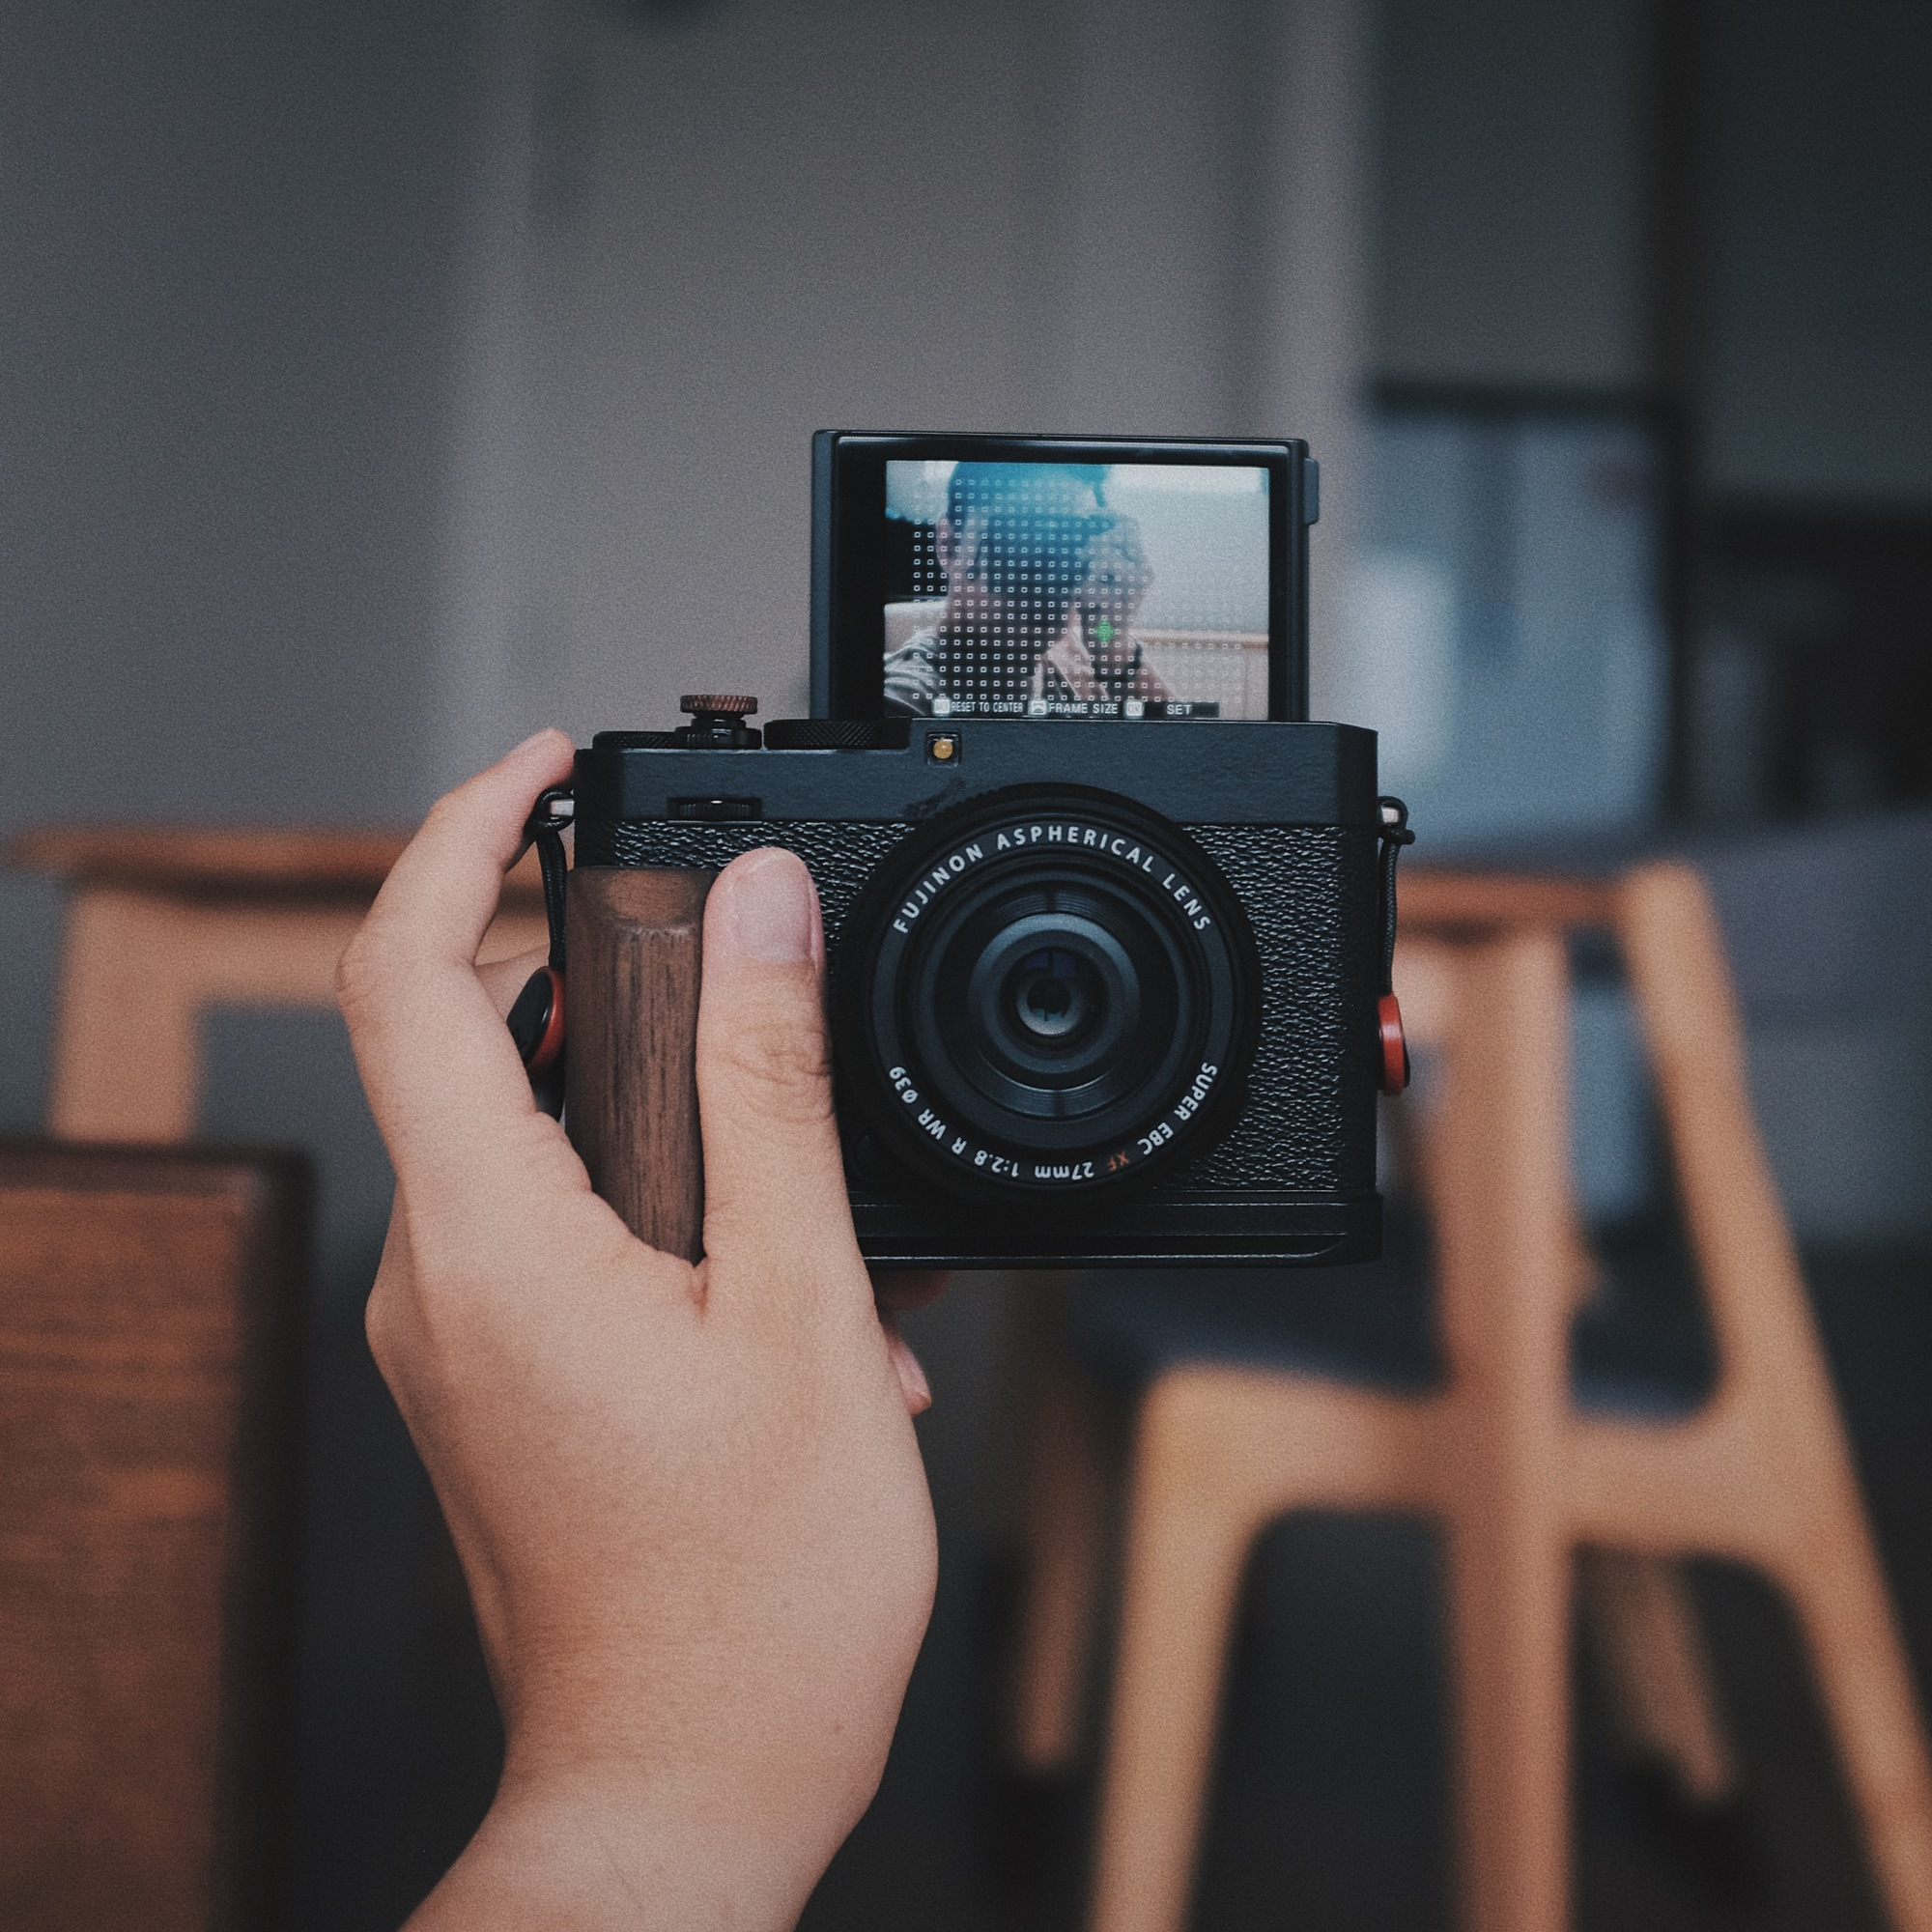
\includegraphics[width=\linewidth]{\envfinaldir/coverpic-prod.jpg}\par
            % \vskip 30pt
            \vfill

            \normalsize\rmfamily\scshape
            \copyright{} The Web Digest Project \hfill\large \envdatestr
        \end{center}
    \end{titlepage}
    % \restoregeometry
}
\newcommand{\simplehref}[1]{%
    \textcolor{blue!80!green}{\href{#1}{#1}}%
}
\renewcommand{\contentsname}{\center\Huge\sffamily\bfseries Contents\par\vskip 20pt}
\newcounter{ipartcounter}
\setcounter{ipartcounter}{0}
\newcommand{\ipart}[1]{
    % \vskip 20pt
    \clearpage
    \stepcounter{ipartcounter}
    \phantomsection
    \addcontentsline{toc}{chapter}{#1}
    % \begin{center}
    %     \Huge
    %     \sffamily\bfseries
    %     #1
    % \end{center}
    % \vskip 20pt plus 7pt
}
\newcounter{ichaptercounter}
\setcounter{ichaptercounter}{0}
\newcommand{\ichapter}[1]{
    % \vskip 20pt
    \clearpage
    \stepcounter{ichaptercounter}
    \phantomsection
    \addcontentsline{toc}{section}{\numberline{\arabic{ichaptercounter}}#1}
    \begin{center}
        \Huge
        \sffamily\bfseries
        #1
    \end{center}
    \vskip 20pt plus 7pt
}
\newcommand{\entrytitlefont}[1]{\subsection*{\raggedright\Large\sffamily\bfseries#1}}
\newcommand{\entryitemGeneric}[2]{
    % argv: title, url
    \parbox{\linewidth}{
        \entrytitlefont{#1}\par\vskip 5pt
        \footnotesize\ttfamily\mdseries
        \simplehref{#2}
    }\vskip 11pt plus 11pt minus 1pt
}
\newcommand{\entryitemGithub}[3]{
    % argv: title, url, desc
    \parbox{\linewidth}{
        \entrytitlefont{#1}\par\vskip 5pt
        \footnotesize\ttfamily\mdseries
        \simplehref{#2}\par\vskip 5pt
        \small\rmfamily\mdseries#3
    }\vskip 11pt plus 11pt minus 1pt
}
\newcommand{\entryitemAp}[3]{
    % argv: title, url, desc
    \parbox{\linewidth}{
        \entrytitlefont{#1}\par\vskip 5pt
        \footnotesize\ttfamily\mdseries
        \simplehref{#2}\par\vskip 5pt
        \small\rmfamily\mdseries#3
    }\vskip 11pt plus 11pt minus 1pt
}
\newcommand{\entryitemHackernews}[3]{
    % argv: title, hnurl, rawurl
    % \parbox{\linewidth}{
    %     \entrytitlefont{#1}\par\vskip 5pt
    %     \footnotesize\ttfamily\mdseries
    %     \simplehref{#3}\par
    %     \textcolor{black!50}{\href{#2}{#2}}
    % }\vskip 11pt plus 11pt minus 1pt
    \begin{minipage}{\linewidth}
            \entrytitlefont{#1}\par\vskip 5pt
            \footnotesize\ttfamily\mdseries
            \simplehref{#3}\par
            \textcolor{black!50}{\href{#2}{#2}}
    \end{minipage}\par\vskip 11pt plus 11pt minus 1pt
}







\begin{document}

\makeheader

\tableofcontents\clearpage




\ipart{Developers}
\ichapter{Hacker News}
\entryitemTwoLinks{Why use mailing lists?}{https://news.ycombinator.com/item?id=45390121}{https://mailarchive.ietf.org/arch/msg/ietf/q6A\_anL1u-Y9iXe-vboiOYamsl0/}

\entryitemTwoLinks{If you are harassed by lasers}{https://news.ycombinator.com/item?id=45389965}{https://www.laserpointersafety.com/harassment.html}

\entryitemTwoLinks{SimpleFold: Folding proteins is simpler than you think}{https://news.ycombinator.com/item?id=45389267}{https://github.com/apple/ml-simplefold}

\entryitemTwoLinks{Modular Manifolds}{https://news.ycombinator.com/item?id=45388728}{https://thinkingmachines.ai/blog/modular-manifolds/}

\entryitemTwoLinks{Open Social}{https://news.ycombinator.com/item?id=45388021}{https://overreacted.io/open-social/}

\entryitemTwoLinks{SpaceX – Evolving the Multi-User Spaceport}{https://news.ycombinator.com/item?id=45387494}{https://www.spacex.com/updates\#multiuser-spaceport}

\entryitemTwoLinks{Fast UDP I/O for Firefox in Rust}{https://news.ycombinator.com/item?id=45387462}{https://max-inden.de/post/fast-udp-io-in-firefox/}

\entryitemTwoLinks{Context is the bottleneck for coding agents now}{https://news.ycombinator.com/item?id=45387374}{https://runnercode.com/blog/context-is-the-bottleneck-for-coding-agents-now}

\entryitemTwoLinks{US cities pay too much for buses}{https://news.ycombinator.com/item?id=45386578}{https://www.bloomberg.com/news/articles/2025-09-26/us-cities-are-paying-too-much-for-new-transit-buses}

\entryitemTwoLinks{Genode OS Framework}{https://news.ycombinator.com/item?id=45384653}{https://genode.org}

\entryitemTwoLinks{Show HN: A little notebook for learning linear algebra with Python}{https://news.ycombinator.com/item?id=45384617}{https://little-book-of.github.io/linear-algebra/books/en-US/lab.html}

\entryitemTwoLinks{Pop OS 24.04 LTS Beta}{https://news.ycombinator.com/item?id=45384481}{https://system76.com/pop/pop-beta/}

\entryitemTwoLinks{Translating a Fortran F-16 Simulator to Unity3D}{https://news.ycombinator.com/item?id=45383637}{https://vazgriz.com/762/f-16-flight-sim-in-unity-3d/}

\entryitemTwoLinks{No reachable chess position with more than 218 moves}{https://news.ycombinator.com/item?id=45382755}{https://lichess.org/@/Tobs40/blog/there-is-no-reachable-chess-position-with-more-than-218-moves/a5xdxeqs}

\entryitemTwoLinks{A platform-jumping prince – History of Prince of Persia's 1990s Ports}{https://news.ycombinator.com/item?id=45382645}{https://www.jordanmechner.com/en/latest-news/\#a-platform-jumping-prince}

\entryitemTwoLinks{Evanston orders Flock to remove reinstalled cameras}{https://news.ycombinator.com/item?id=45382434}{https://evanstonroundtable.com/2025/09/24/flock-safety-reinstalls-evanston-cameras/}

\entryitemTwoLinks{My Deus Ex lipsyncing fix mod}{https://news.ycombinator.com/item?id=45382397}{https://www.joewintergreen.com/my-deus-ex-lipsyncing-fix-mod-making-of/}

\entryitemTwoLinks{Britain to introduce compulsory digital ID for workers}{https://news.ycombinator.com/item?id=45381810}{https://www.reuters.com/world/uk/britain-introduce-mandatory-digital-id-cards-2025-09-26/}

\entryitemTwoLinks{Exploit allows for takeover of fleets of Unitree robots}{https://news.ycombinator.com/item?id=45381590}{https://spectrum.ieee.org/unitree-robot-exploit}

\entryitemTwoLinks{Investigating a Forged PDF}{https://news.ycombinator.com/item?id=45381010}{https://mjg59.dreamwidth.org/73317.html}\ichapter{Phoronix}
\entryitemGeneric{\hskip 0pt{}Ubuntu 25.10's Only Supported RISC-V Platform: QEMU Virtualization}{https://www.phoronix.com/news/Ubuntu-25.10-RISC-V-QEMU}

\entryitemGeneric{\hskip 0pt{}Features Expected For Linux 6.18: File-System Improvements, Sheaves, New Drivers \& More Perf}{https://www.phoronix.com/news/Linux-6.18-Features-Expected}

\entryitemGeneric{\hskip 0pt{}Vulkan 1.4.328 Published With Copy Memory Indirect Extension}{https://www.phoronix.com/news/Vulkan-1.4.328}

\entryitemGeneric{\hskip 0pt{}Linux 6.17 Gets Ready For Release With Intel Panther Lake \& More Performance}{https://www.phoronix.com/news/Linux-6.17-Features-Reminder}

\entryitemGeneric{\hskip 0pt{}Ubuntu 25.10's Move To Rust Coreutils Is Causing Major Breakage For Some Executables}{https://www.phoronix.com/news/Ubuntu-25.10-Coreutils-Makeself}

\entryitemGeneric{\hskip 0pt{}Time Is Running Out On Our Autumn Deal To Help Support Linux Hardware Reviews}{https://www.phoronix.com/news/Autumn-2025-Deal-Ending-Soon}

\entryitemGeneric{\hskip 0pt{}Intel Returns To Working On The Habana Labs AI Accelerator Linux Driver}{https://www.phoronix.com/news/Intel-Habana-Labs-6.18-Return}

\entryitemGeneric{\hskip 0pt{}Linux 6.18 Landing Patch For Old AMD Bulldozer CPUs With XOP Instruction Set}{https://www.phoronix.com/news/Linux-6.18-AMD-Bulldozer-XOP}

\entryitemGeneric{\hskip 0pt{}Mesa 25.3 Intel Driver Lands Support For Stochastic Rounding}{https://www.phoronix.com/news/Mesa-Intel-Stochastic-Rounding}


\ipart{Developers~~~~(zh-Hans)}
\ichapter{Solidot}
\entryitemGeneric{\hskip 0pt{}在笔记本电脑上模拟宇宙}{https://www.solidot.org/story?sid=82428}

\entryitemGeneric{\hskip 0pt{}ROG Xbox Ally X 售价 1000 美元}{https://www.solidot.org/story?sid=82427}

\entryitemGeneric{\hskip 0pt{}OpenAI 准备建造的数据中心消耗的电力相当于纽约和圣迭戈 }{https://www.solidot.org/story?sid=82426}

\entryitemGeneric{\hskip 0pt{}微软禁止以色列国防部使用它的某些云服务}{https://www.solidot.org/story?sid=82425}

\entryitemGeneric{\hskip 0pt{}对 117 岁寿星的 DNA 研究揭示了长寿的线索}{https://www.solidot.org/story?sid=82423}

\entryitemGeneric{\hskip 0pt{}中国学者《科学》论文接受率为北美同行 1/4}{https://www.solidot.org/story?sid=82422}

\entryitemGeneric{\hskip 0pt{}定期锻炼有助于重塑控制心脏的神经}{https://www.solidot.org/story?sid=82421}

\entryitemGeneric{\hskip 0pt{}英特尔与苹果洽谈投资和加强合作}{https://www.solidot.org/story?sid=82420}

\entryitemGeneric{\hskip 0pt{}微软将让 Copilot 在用户注视下控制浏览器完成各种任务}{https://www.solidot.org/story?sid=82419}

\entryitemGeneric{\hskip 0pt{}俄罗斯卫星带着 75 只老鼠 1500 只果蝇返回地面}{https://www.solidot.org/story?sid=82418}

\entryitemGeneric{\hskip 0pt{}人类骨骼内部发现微塑料}{https://www.solidot.org/story?sid=82417}

\entryitemGeneric{\hskip 0pt{}中国科学家基于不倒翁结构设计扑翼微飞行器}{https://www.solidot.org/story?sid=82416}

\entryitemGeneric{\hskip 0pt{}安理会讨论 AI 和平利用与风险}{https://www.solidot.org/story?sid=82415}

\entryitemGeneric{\hskip 0pt{}智能手机摄像头能变成高光谱传感器}{https://www.solidot.org/story?sid=82414}

\entryitemGeneric{\hskip 0pt{}微软为美国和欧洲的 Windows 10 用户提供免费安全更新一年,只要他们用 MS 账号登陆}{https://www.solidot.org/story?sid=82413}

\entryitemGeneric{\hskip 0pt{}NASA 宣布计划明年 2 月发射宇航员绕月球飞行}{https://www.solidot.org/story?sid=82412}

\entryitemGeneric{\hskip 0pt{}Instagram 月活用户数突破 30 亿}{https://www.solidot.org/story?sid=82411}

\entryitemGeneric{\hskip 0pt{}日本丰明议会通过了每天限制智能手机使用时间在两小时内的法令}{https://www.solidot.org/story?sid=82410}

\entryitemGeneric{\hskip 0pt{}OpenSSF 警告开源基础设施不能运行在祈祷之上}{https://www.solidot.org/story?sid=82409}

\entryitemGeneric{\hskip 0pt{}AI 生成大量劣质重复性研究}{https://www.solidot.org/story?sid=82408}\ichapter{V2EX}
\entryitemGeneric{\hskip 0pt{}[推广] AI 作曲要干掉乐队了? Suno v5 实测}{https://www.v2ex.com/t/1162148}

\entryitemGeneric{\hskip 0pt{}[程序员] 想问下有人用过 kafka streams 吗}{https://www.v2ex.com/t/1162146}

\entryitemGeneric{\hskip 0pt{}[分享发现] 现在的闲鱼二手手机比全新还贵}{https://www.v2ex.com/t/1162145}

\entryitemGeneric{\hskip 0pt{}[iPhone] iPhone 17Pro 机器连接某些 wifi 网络时会不停重启}{https://www.v2ex.com/t/1162144}

\entryitemGeneric{\hskip 0pt{}[V2EX] 关于通过 Solana 注册新账号与设置密码的一些想法}{https://www.v2ex.com/t/1162142}

\entryitemGeneric{\hskip 0pt{}[酷工作] [杭州] [阿里云] AI 业务团队招人}{https://www.v2ex.com/t/1162141}

\entryitemGeneric{\hskip 0pt{}[程序员] [车已开]Claude MAX 20X 5=3 英国移动网络中转}{https://www.v2ex.com/t/1162140}

\entryitemGeneric{\hskip 0pt{}[Android] moto 的 myui 会杀 fcm 进程嘛}{https://www.v2ex.com/t/1162139}

\entryitemGeneric{\hskip 0pt{}[问与答] 隔壁看到个帖子, 如果我遇到也不知道怎么办}{https://www.v2ex.com/t/1162138}

\entryitemGeneric{\hskip 0pt{}[分享创造] 专为浏览器扩展开发而设计的 React Portal}{https://www.v2ex.com/t/1162137}

\entryitemGeneric{\hskip 0pt{}[问与答] 大佬们,到底应该怎么准备面试啊}{https://www.v2ex.com/t/1162136}

\entryitemGeneric{\hskip 0pt{}[分享发现] Symposium: Rust 核心开发者怎么用 AI agent}{https://www.v2ex.com/t/1162135}

\entryitemGeneric{\hskip 0pt{}[程序员] 京东买的 MacBook,保修日期不是我激活的一年后,电池循环次数也不是 0,是正常吗}{https://www.v2ex.com/t/1162134}

\entryitemGeneric{\hskip 0pt{}[分享创造] 🎁 福利:[内购限免+\$V2EX 打赏]新作品 2Camera 发布啦!前后双摄,双重拍摄相机 📷}{https://www.v2ex.com/t/1162133}

\entryitemGeneric{\hskip 0pt{}[Apple] 想重回苹果,目前有一两个痛点请帮我解决一下}{https://www.v2ex.com/t/1162132}

\entryitemGeneric{\hskip 0pt{}[Solana] 买理想送 V 币}{https://www.v2ex.com/t/1162129}

\entryitemGeneric{\hskip 0pt{}[Apple] 钱迹用了 1968 天了,今天开了终身会员,开心}{https://www.v2ex.com/t/1162128}

\entryitemGeneric{\hskip 0pt{}[macOS] 观小火箭最新版支持显示在菜单栏的帖子,然后更新出 bug 了}{https://www.v2ex.com/t/1162127}

\entryitemGeneric{\hskip 0pt{}[电动汽车] 有没有理想的 v 友车主,这个牌子的车咋样。。。看到 i6 的发布会,挺不错}{https://www.v2ex.com/t/1162126}

\entryitemGeneric{\hskip 0pt{}[macOS] touch id}{https://www.v2ex.com/t/1162125}

\entryitemGeneric{\hskip 0pt{}[程序员] 你知道你的 coding agent 的提示词里都有什么吗}{https://www.v2ex.com/t/1162124}

\entryitemGeneric{\hskip 0pt{}[iPhone] iPhone 17 发热到烫手的解决方案}{https://www.v2ex.com/t/1162122}

\entryitemGeneric{\hskip 0pt{}[生活] 大家有没有身边的 2 类套中人}{https://www.v2ex.com/t/1162121}

\entryitemGeneric{\hskip 0pt{}[macOS] 马勒戈壁的, SB Parallels Desktop for Mac,我都订阅到 2029 年,升级一下就不行了?不能激活!}{https://www.v2ex.com/t/1162120}

\entryitemGeneric{\hskip 0pt{}[微信] 请教一个微信的公众号/小程序流量主广告规则,是不是这样}{https://www.v2ex.com/t/1162119}

\entryitemGeneric{\hskip 0pt{}[macOS] Parallels Desktop for Mac 26.10 版本出大问题! 升级之后无法激活许可证}{https://www.v2ex.com/t/1162118}

\entryitemGeneric{\hskip 0pt{}[职场话题] 吐槽一下失业金申领}{https://www.v2ex.com/t/1162116}

\entryitemGeneric{\hskip 0pt{}[分享创造] 创业到草根}{https://www.v2ex.com/t/1162115}

\entryitemGeneric{\hskip 0pt{}[生活] 今天在小区的缴费处遇到了小时候的玩伴}{https://www.v2ex.com/t/1162113}

\entryitemGeneric{\hskip 0pt{}[分享创造] Archrome 是一款受 Arc 浏览器启发的 Chrome 扩展程序.}{https://www.v2ex.com/t/1162111}

\entryitemGeneric{\hskip 0pt{}[Android] 现在的安卓机在无法 ROOT 的情况下还能安装 CA 证书吗}{https://www.v2ex.com/t/1162109}

\entryitemGeneric{\hskip 0pt{}[Solana] 新手学习,原来 V 币转成 SOL 必须还得有 SOL 余额用来抵扣手续费}{https://www.v2ex.com/t/1162108}

\entryitemGeneric{\hskip 0pt{}[上海] 坐标上海宝山淞南, 诚聘育儿嫂, 薪资在 7~8k}{https://www.v2ex.com/t/1162107}

\entryitemGeneric{\hskip 0pt{}[问与答] 请问这个域名是爱他美官方的吗?}{https://www.v2ex.com/t/1162106}

\entryitemGeneric{\hskip 0pt{}[推广] 教育 AIGC 创造力社群}{https://www.v2ex.com/t/1162105}

\entryitemGeneric{\hskip 0pt{}[耳机] 大家有没有合适的降噪耳机推荐?}{https://www.v2ex.com/t/1162103}

\entryitemGeneric{\hskip 0pt{}[问与答] airpods 歌曲标记为喜欢有什么快捷操作 or 办法么?}{https://www.v2ex.com/t/1162102}

\entryitemGeneric{\hskip 0pt{}[iPhone] iPhone 现在的价格只有我觉得贵吗?}{https://www.v2ex.com/t/1162101}

\entryitemGeneric{\hskip 0pt{}[酷工作] [社招] [抖音] [上海/北京] 推荐架构工程师--在线方向}{https://www.v2ex.com/t/1162100}

\entryitemGeneric{\hskip 0pt{}[分享发现] 1Password 又送一年}{https://www.v2ex.com/t/1162099}

\entryitemGeneric{\hskip 0pt{}[Cursor] 请教一下, cursor 会卡住}{https://www.v2ex.com/t/1162098}

\entryitemGeneric{\hskip 0pt{}[程序员] chatgpt 的翻译还真是接地气。。。}{https://www.v2ex.com/t/1162096}

\entryitemGeneric{\hskip 0pt{}[问与答] 中美就妥善解决 TikTok 问题达成基本框架共识}{https://www.v2ex.com/t/1162095}

\entryitemGeneric{\hskip 0pt{}[问与答] 请问农村自建房大家用什么净水器方案啊}{https://www.v2ex.com/t/1162093}

\entryitemGeneric{\hskip 0pt{}[酷工作] [内推] [广州] [世界 500 强外企] WAF 安全工程师}{https://www.v2ex.com/t/1162092}

\entryitemGeneric{\hskip 0pt{}[Apple] iPhone 看通知时的亮屏逻辑,困扰}{https://www.v2ex.com/t/1162091}

\entryitemGeneric{\hskip 0pt{}[深圳] 求一个深圳本土的组装电脑公司联系方式。}{https://www.v2ex.com/t/1162090}

\entryitemGeneric{\hskip 0pt{}[知乎] 逆天知乎,挂在浏览器后台不知不觉就占了 12.8GB 内存……}{https://www.v2ex.com/t/1162089}

\entryitemGeneric{\hskip 0pt{}[投资] 港美券商还有能开的吗?}{https://www.v2ex.com/t/1162088}

\entryitemGeneric{\hskip 0pt{}[分享发现] Nano banana 图片生成|国内极简无障碍版}{https://www.v2ex.com/t/1162087}


\ipart{Generic News}







\clearpage
\leavevmode\vfill
\footnotesize

Copyright \copyright{} 2023-2025 Neruthes and other contributors.

This document is published with CC BY-NC-ND 4.0 license.

The entries listed in this newsletter may be copyrighted by their respective creators.

This newsletter is generated by the Web Digest project.

The newsletters are also delivered via Telegram channel \CJKunderline{\href{https://t.me/webdigestchannel}{https://t.me/webdigestchannel}}.\\
RSS feed is available at \CJKunderline{\href{https://webdigest.pages.dev/rss.xml}{https://webdigest.pages.dev/rss.xml}}.

This newsletter is available in PDF at
\CJKunderline{\href{https://webdigest.pages.dev/}{https://webdigest.pages.dev/}}.

The source code being used to generate this newsletter is available at\\
\CJKunderline{\href{https://github.com/neruthes/webdigest}{https://github.com/neruthes/webdigest}}.

This newsletter is also available in
\CJKunderline{\href{http://webdigest.pages.dev/readhtml/\envyear/WebDigest-20250927.html}{HTML}} and
\CJKunderline{\href{https://github.com/neruthes/webdigest/blob/master/markdown/\envyear/WebDigest-20250927.md}{Markdown}}.


\coverpic{https://unsplash.com/photos/two-people-pose-for-the-camera-in-cool-outfits-Zsvdjmg0Ato}{LOGAN WEAVER | @LGNWVR}


\end{document}
